\documentclass{article}
\usepackage{iclr2026_conference,times}

\input{math_commands.tex}

\usepackage{hyperref}
\usepackage{url}
\usepackage{graphicx}

\title{Low-Rank Networks: Loss Landscape Valley--Frequency Correspondence}

% Authors must not appear in the submitted version.
\author{Anonymous Author(s)
}

%\iclrfinalcopy
\begin{document}

\maketitle

\begin{abstract}
We study the \textbf{relation between feature learning and the loss landscape} for low-rank neural networks trained on frequency-dependent, 1D regression targets. In controlled experiments (matrix-rank nets, sum-of-cosines target, adaptive LR schedule), we observe that: (1) the loss exhibits a \emph{plateau--sharp--plateau} structure where each plateau (or saddle region) corresponds to a frequency band to be learned and the dynamics are \emph{saddle-to-saddle}, so each sharp transition coincides with the network capturing a new frequency and with more oscillatory partial functions (e.g.\ layer $L$ developing on the order of $2L$ spikes, not observed in standard MLPs); (2) the landscape appears as a \emph{plateau with many sharp, deep basins} that are hard to enter unless the learning rate is small---at each LR divide the loss drops sharply and the trajectory descends into such a basin, with visible refinement of internal representations (we report loss, fit, and partial functions before/after LR divides); (3) scaling of plateau-escape time with learning rate and batch size, and sensitivity of the lower landscape to sample size $N$, are consistent with the picture that the landscape is aligned with hierarchical feature acquisition. We provide a clear methodology and reproducible configs. Scope: 1D regression and the sumcos/MMNN setting. This submission fits the workshop's focus on empirical studies of loss landscapes and learned representations.
\end{abstract}

\section{Introduction}
\label{sec:intro}

A central question in deep learning is how the \textbf{geometry of the loss landscape} (plateaus, sharp transitions, basins) connects to \textbf{what the network learns} (channel-wise representations, frequency bands, oscillatory structure). For low-rank neural networks, this connection is still poorly understood. In this paper we provide a focused empirical study of the \textbf{relation between feature learning and the loss landscape} in such networks, in a setting chosen for controllability and reproducibility.

We use matrix-rank neural networks (MMNNs) and a 1D frequency-dependent target (sum of cosines) so that both the loss curve and the evolution of partial functions (channel outputs) can be measured and compared. Our main observations are: (i) the loss exhibits a plateau--sharp--plateau structure where each plateau (or saddle) corresponds to a frequency to be learned and the dynamics are saddle-to-saddle, so each sharp drop coincides with the acquisition of a new frequency and with more oscillatory partial functions; (ii) the landscape behaves like a plateau with many sharp, deep basins that are hard to reach unless the learning rate is small---at each LR divide the loss drops sharply and we show loss, fit, and partial functions before and after LR divides to make this link explicit; (iii) observables such as the number of minima per channel and the $2L$-spike pattern per layer $L$ provide a concrete bridge between landscape and feature learning. We give a clear methodology (Section~\ref{sec:architecture}--\ref{sec:methodology}), including the rationale for 1D data and full experimental protocol, and we provide config files and script paths so that results can be reproduced or extended. \textbf{Scope and limitations:} the study is restricted to 1D regression and the sumcos/MMNN setting; we do not claim that the same relation holds in higher dimensions or for other architectures without further experiments. The takeaway for the reviewer is that \emph{in this setting}, understanding the loss landscape amounts to understanding how and when features are acquired, and that the relation is testable via the provided methodology.

\section{Architecture and target}
\label{sec:architecture}

\subsection{Target and data}
The target is $y(x) = \sum_{k=1}^{\mathrm{factor}} \cos(2\pi k x)$ on $x \in [-1,1]$ (\texttt{target\_baseline} in \texttt{run\_scaling\_law\_depth\_width.py}). For \textbf{factor $= 3$} ($f_3$), $y(x) = \cos(2\pi x) + \cos(4\pi x) + \cos(6\pi x)$. Training inputs are a uniform grid of $N_{\mathrm{train}}$ points; for the reported figures we use $N_{\mathrm{train}} = 768$ and batch size $8$. Loss is MSE. In broader baseline sweeps (factor 1--5, $N = \mathrm{base} \times \mathrm{factor}$, ranks 5 and 10, batch sizes 1--16; see \texttt{BASELINE\_SWEEP\_SETUPS\_AND\_RANKS.md} for batch-size analysis), ``worked'' configs (test error $< 0.01$) are 73 for rank 10 and 76 for rank 5 out of 429 and 750 completed runs respectively. \textbf{Main conclusion from the full run:} small batch (1, 2, 4) consistently outperforms large batch (8, 16); for rank 5, small bs is optimal and depth $L=3$ leads to better results than $L=2$ in the regimes tested. Small batch always performs better in these sweeps, consistent with plateau escape and basin access depending on gradient noise and LR.

\subsection{MMNN architecture}
The model is a \textbf{matrix-rank neural network (MMNN)}: input and output dimension $1$; hidden layers have \textbf{rank} $R$ and \textbf{width} $W$. For depth $L$, the layer sequence is $1 \to R \to W \to R \to W \to \cdots \to R \to 1$: each ``layer'' is (i) a linear map rank$\to$width, (ii) ReLU, (iii) a linear map width$\to$rank, so there are $L$ such blocks. In the reported configs, $W = 1024$, $R = 10$, and $L \in \{2, 3\}$. With \textbf{fixWb = True}, the first linear (rank$\to$width) in each block is \emph{frozen}; only the width$\to$rank linears and their biases are trained (low-rank channel weights). Initialization is $\mu$-parameterization: weights uniform in $[-1,1]$ then scaled by $1/\sqrt{\mathrm{rank}}$ or $1/\sqrt{\mathrm{width}}$ as appropriate. Optimizer is SGD with momentum $0$ and gradient clipping (max norm $1.0$).

\section{Methodology}
\label{sec:methodology}

\subsection{Why 1D data}
We use \textbf{1-dimensional} regression for three reasons that are standard in mean-field and optimization analyses of low-rank networks. \textbf{(i) Mean-field parameterization and convergence of $\E_Z[\cdot]$:} the training dynamics in the mean-field width limit are expressed in terms of expectations over the data distribution, $\E_Z[\cdot]$. With 1D input we can use \emph{large sample sizes} (e.g.\ $N_{\mathrm{train}} = 768$ or several thousand) so that empirical averages over the training set approximate these expectations well; optimization dynamics are then not confounded by overfitting or sample-complexity effects, and the finite-width behavior is close to the mean-field limit. \textbf{(ii) Controlled hierarchical frequency learning:} a frequency-dependent target on $[-1,1]$ (e.g.\ sum of cosines) provides a controlled setting to study how the loss landscape and feature learning interact across frequency bands---with a direct link to tractable toy models (e.g.\ two-point support) and to the interpretation that each sharp loss drop corresponds to capturing a new frequency. \textbf{(iii) Interpretability:} 1D allows clear visualization and quantification of channel specialization (spatial location and frequency) and of observables such as the log-ratio evolution and the number of minima per partial-function component.

\subsection{Training protocol and observables}
The initial learning rate is $10^{-2}$. The schedule is \textbf{adaptive stagnation}: over a sliding window of 10 epochs, if the mean training loss does not improve compared to the previous window, and at least 20 epochs have passed since the last reduction, the learning rate is replaced by the next value in a precomputed sequence (divide by $2$ each step, 25 steps; training stops if LR falls below $10^{-6}$). At each LR reduction, the script saves (i) the model state \emph{just before} the divide and (ii) the state \emph{10 epochs after} the divide. The reported figures compare these checkpoints: \textbf{loss} (training curve), \textbf{fit} (prediction vs.\ target), and \textbf{partial functions} (channel outputs at selected layers). Max epochs 10,000; seed 42. The Appendix gives full experiment methodology and all configs.

\section{Plateau--sharp--plateau and frequency structure}
\label{sec:plateau}

In our experiments, the training loss consistently exhibits long \emph{plateaus} interrupted by \emph{sharp} drops. We interpret this as follows: each plateau (or saddle region) corresponds to a \emph{frequency band} that has not yet been learned; the dynamics move \emph{saddle-to-saddle}, so the training trajectory is directly tied to \emph{frequency learning}---each sharp transition marks the acquisition of a new frequency. Initially the predictor is nearly constant and the loss is flat; after an epoch count that depends strongly on the learning rate, a first sharp transition occurs---for lr $10^{-2}$ we observe a plateau of on the order of \textbf{20 epochs} before the first drop, versus hundreds to thousands of epochs for lr $10^{-4}$. \textbf{Feature--landscape link:} we observe that each such transition coincides with the network capturing a new frequency band and with the internal partial functions (channel outputs) gaining more oscillatory structure---e.g.\ an increase in the mean number of strict local minima per component in deeper layers. The landscape thus displays a hierarchical structure aligned with hierarchical feature learning: low-to-high frequency in the target is reflected in staged refinement of the learned representation.

Early in training, many parameter directions give similar loss (landscape appears flat in those directions). Low-rank parameterizations reduce the number of effective directions, which we hypothesize makes the landscape more structured and interpretable in terms of the $r$ channels. After plateaus, the dynamics can be described as entering a favorable basin; learning-rate reduction at the right time triggers this descent and, with it, a visible change in the partial functions (Section~\ref{sec:figures}).

\section{Learning rate and sharp basins on a plateau}
\label{sec:lr}

The loss drops \emph{sharply and almost instantaneously} at each learning-rate (LR) divide in our runs (Figures~\ref{fig:loss_fit_L2} and \ref{fig:loss_fit_L3}). This suggests that the landscape has \textbf{very sharp basins}---deep, narrow holes---sitting on top of a plateau: the trajectory wanders on the plateau until LR is reduced, at which point it can descend into one of these holes and the loss falls abruptly. Thus the picture is a \emph{plateau with many sharp holes that are hard to enter unless the learning rate is small}; with large LR the optimizer overshoots or fails to settle into these basins. \textbf{Feature--landscape link:} entering such a basin is accompanied by a visible refinement of the learned features: the partial functions before vs.\ after an LR divide (Figure~\ref{fig:partial_L3}) show how internal representations change when the trajectory drops into a sharper basin. After long plateaus, the landscape appears to contain multiple such basins that are not accessible in the initial phase; a learning rate that is too large may prevent the trajectory from entering them and thus from reaching the feature configurations that support low loss. This is consistent with \emph{grokking}-like phenomena, where generalization improves after prolonged training once the dynamics enter a favorable basin and the corresponding feature structure is acquired.

\section{Adam, EOS jump, and instability}
\label{sec:adam}

In our setting, Adam training is observed to be highly unstable. A notable empirical finding is that a \emph{jump} in the trajectory near \emph{end-of-schedule} (EOS) can land the solution in a sharp but small basin---in some runs with a shape resembling multiple local minima and the global minimum in the middle. When such a jump occurs at EOS, the optimizer effectively reaches a favorable basin; this may partly explain why Adam can perform well in practice despite instability. The \emph{lower part} of the landscape (near good minima) appears more sensitive to the number of samples $N$ than the upper part; under unstable or very long training, behavior can exhibit unexpected sensitivity or non-monotonicity. When instability is present, training curves sometimes display a characteristic symmetry; we leave a systematic characterization for future work.

\subsection{Symmetry preservation: low-rank vs full-rank}
\label{sec:symmetry}

Targets such as $y(x)=\sum_k \cos(2\pi k x)$ or $f(x)=\cos(f_1\pi x^2)-0.8\cos(f_2\pi x^2)$ on $[-1,1]$ are \textbf{symmetric about $x=0$} (even in $x$). Under batched optimization, full-rank (MLP) networks can learn \emph{asymmetric} internal representations for these symmetric targets; low-rank (RF-LR or MMNN) networks, in contrast, tend to \textbf{preserve symmetry} in the channel partials and activations. Figure~\ref{fig:mlp-asymmetry} shows the asymmetry when the random-feature/low-rank structure is removed: at layers 7 and 16, the learned features are visibly asymmetric about $x=0$ (same setup as symmetric low-rank runs: 8 layers, $n=1024$, $r=20$, target $(f_1,f_2)=(144,48)$, $N=4k$, Adam, batch 100). So the low-rank constraint acts as an \emph{implicit regularizer} that preserves the target's geometric symmetry and restricts the trajectory to basins whose minimizers exhibit symmetric feature structure; full-rank nets can fall into asymmetric basins that still achieve low loss. This fits the valley--frequency picture: the landscape for low-rank nets appears to have a symmetry-aligned structure that full-rank nets do not respect.

\begin{figure}[htbp]
\centering
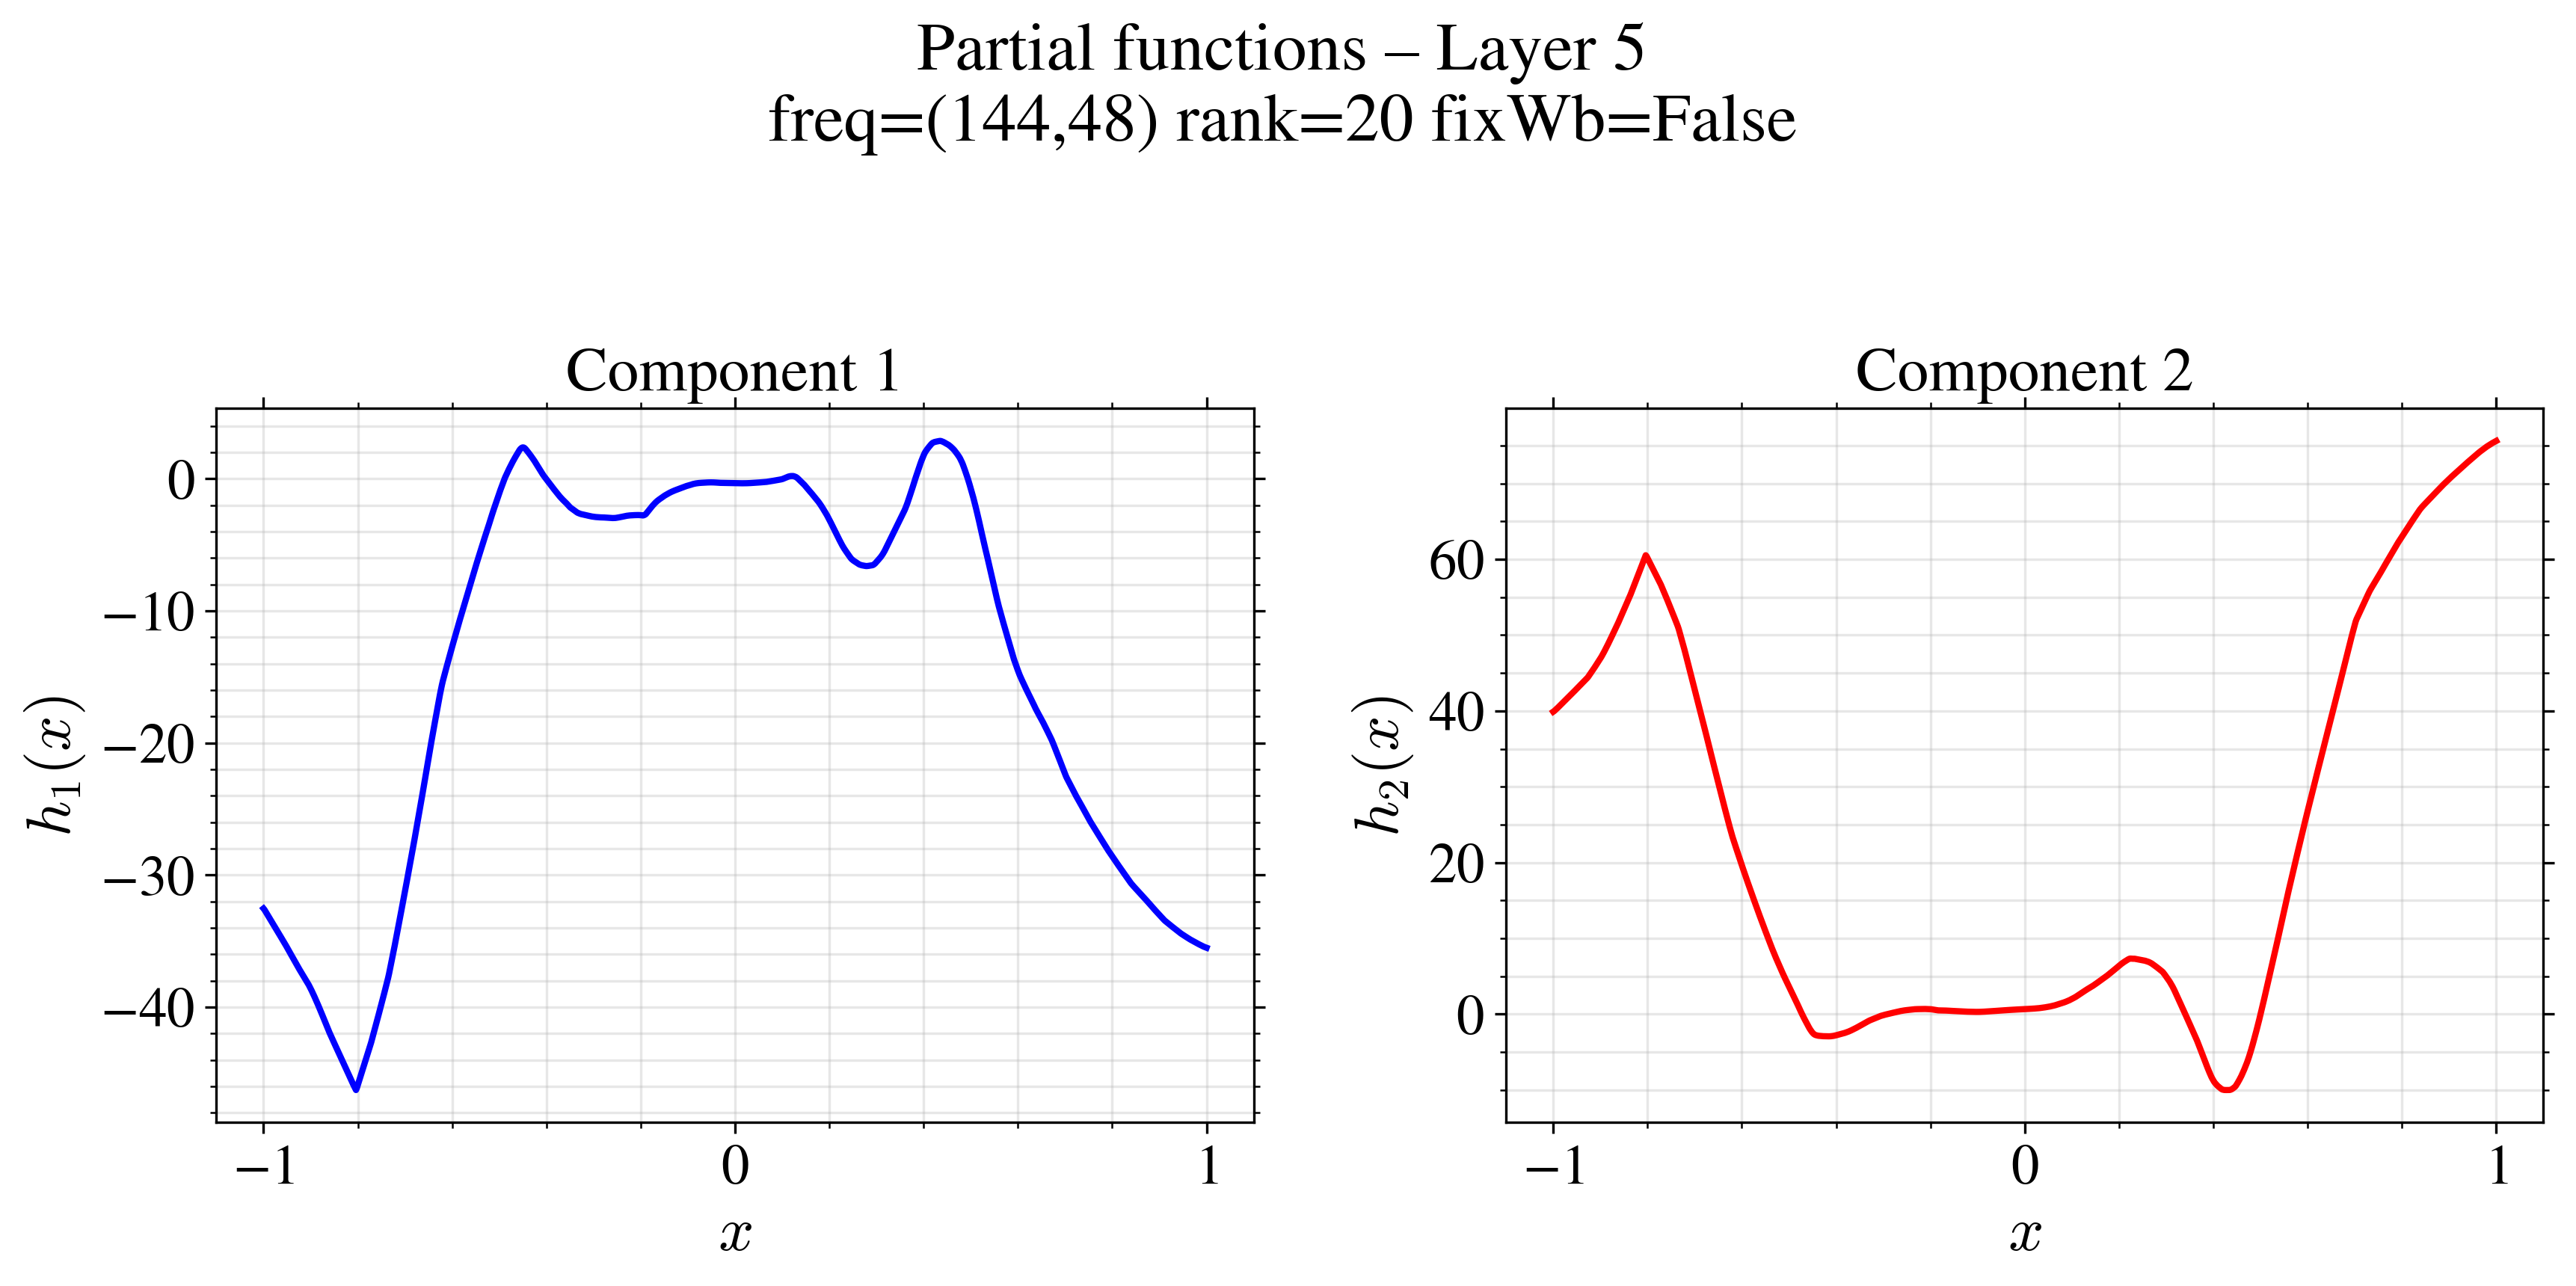
\includegraphics[width=0.42\linewidth]{figures/mlp_asymmetry_layer7.png}\hfill
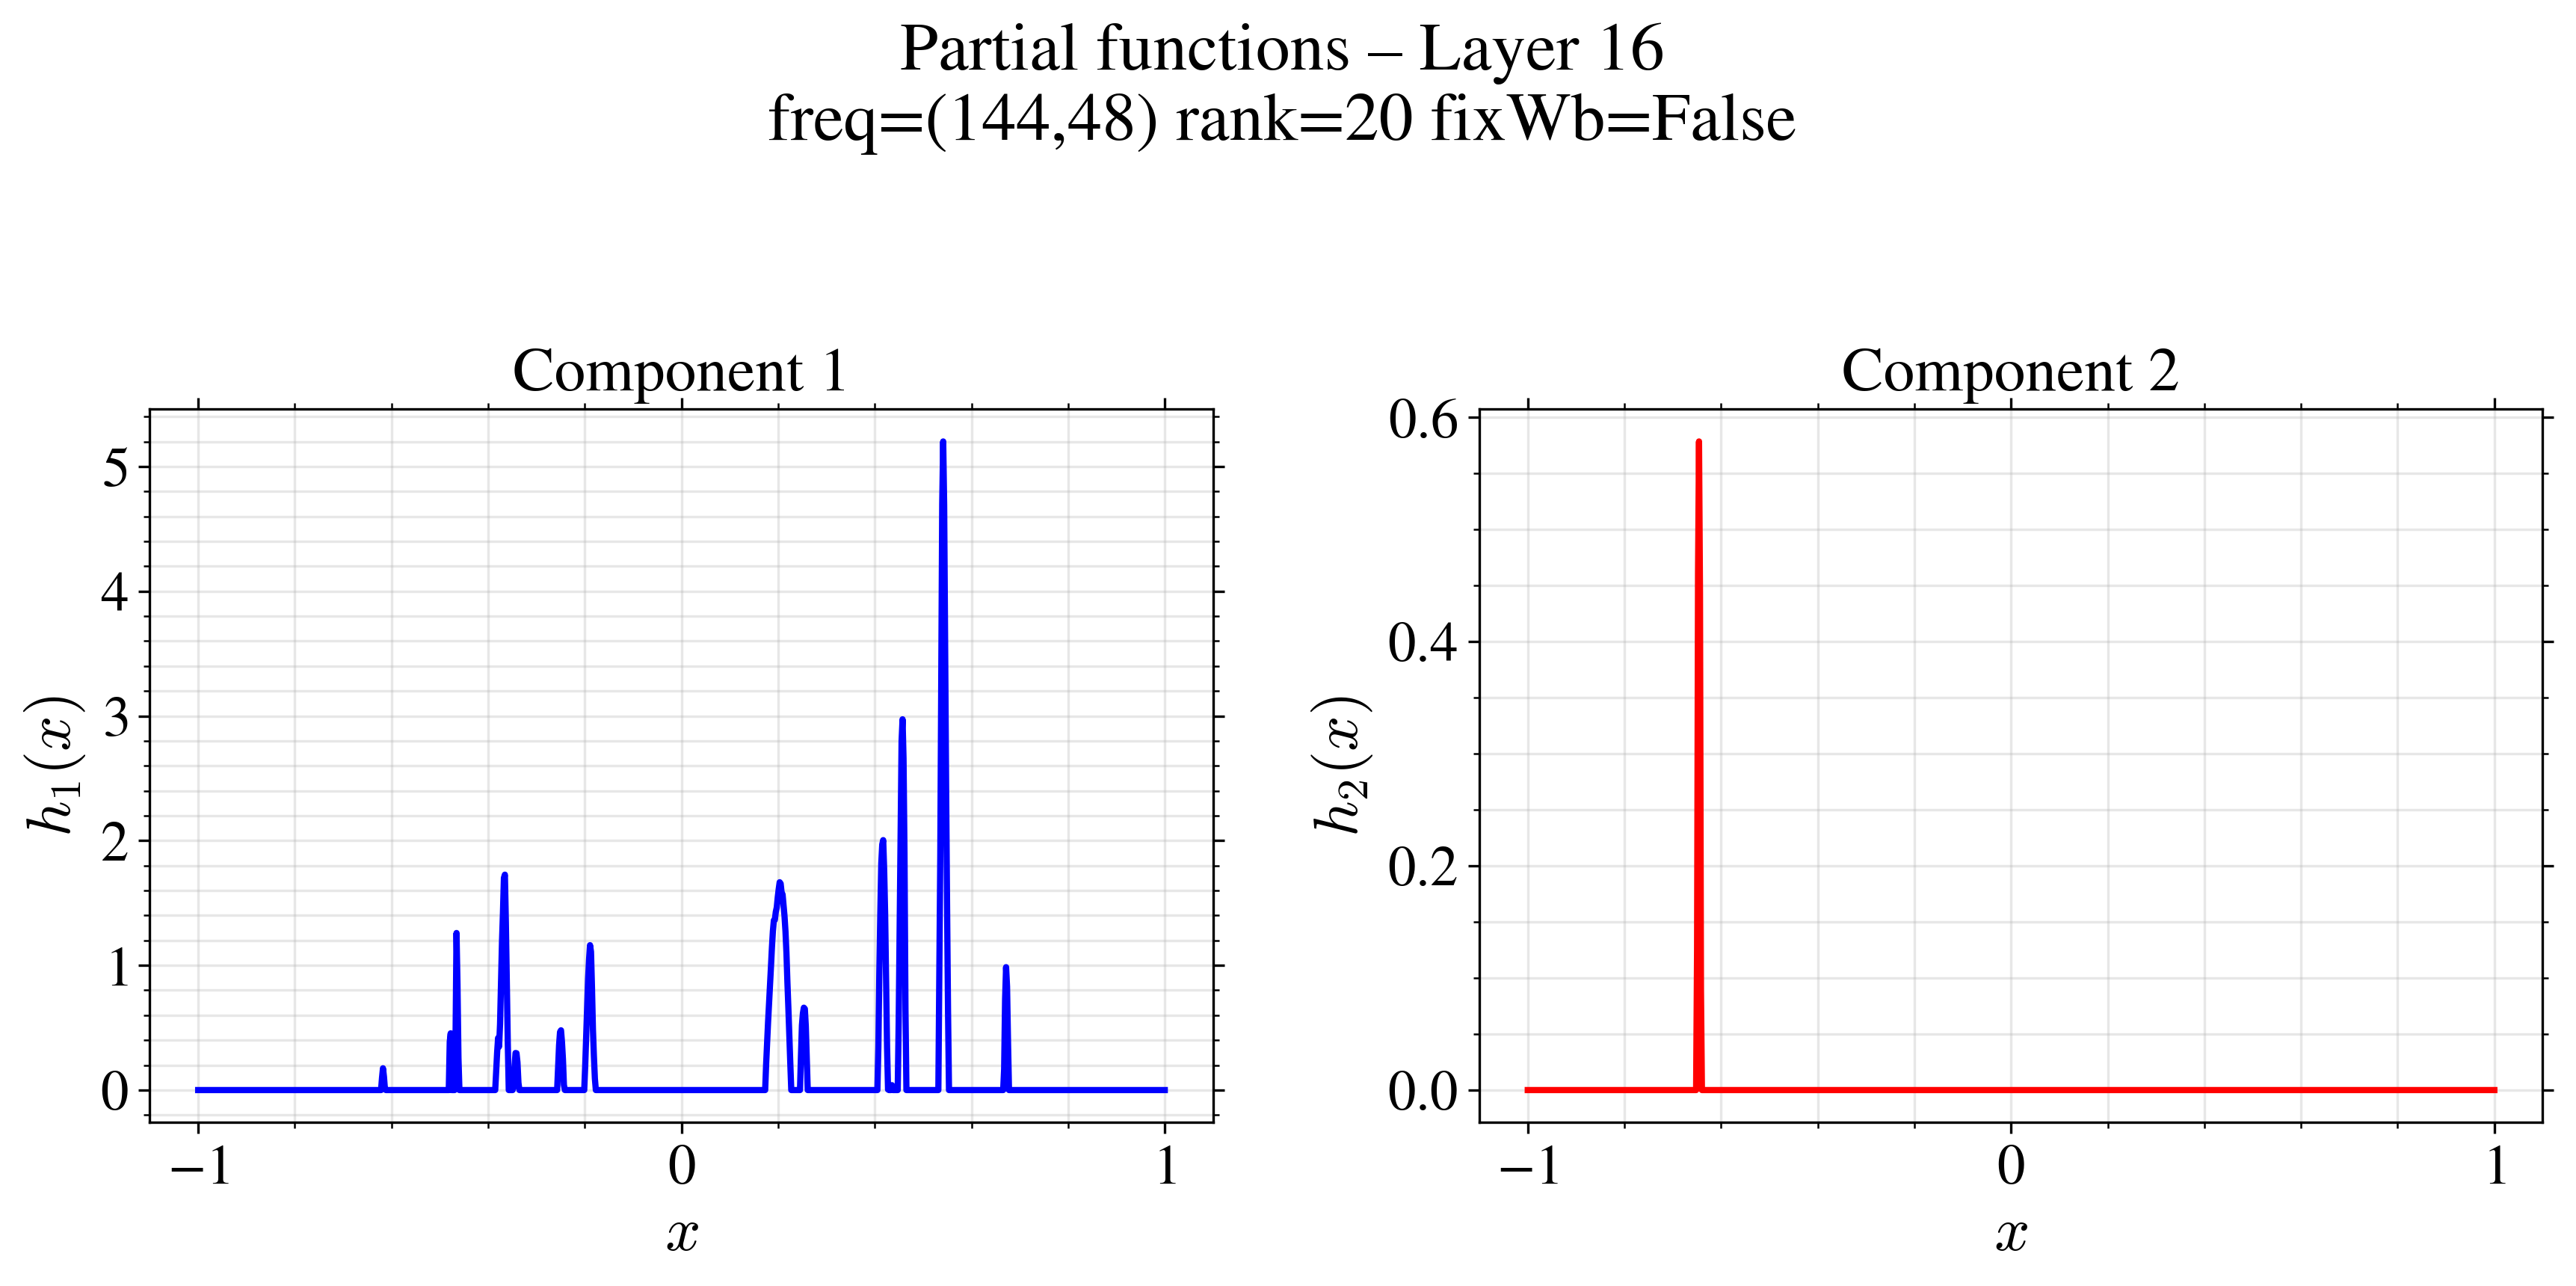
\includegraphics[width=0.42\linewidth]{figures/mlp_asymmetry_layer16.png}
\caption{Symmetry comparison: asymmetry when RF/low-rank is removed (full-rank MLP). (a) Layer 7. (b) Layer 16. $r=20$, target $(f_1,f_2)=(144,48)$; full-rank learns asymmetric features despite symmetric target; low-rank (not shown here) preserves symmetry. Source: \texttt{icml\_sgdadamlandscapedynamical/tofill.tex}.}
\label{fig:mlp-asymmetry}
\end{figure}

\section{Scaling and the feature--landscape relation}
\label{sec:scaling}

Scaling dimensions that affect both the loss landscape and feature learning in our experiments include the following. \textbf{Depth and width:} we observe that layer $L$ can exhibit on the order of $2L$ spikes (or similar oscillatory structure) in the partial functions, a pattern not observed in standard MLPs and thus a distinctive feature-learning signature of low-rank architectures that is tied to the hierarchical loss landscape (deeper layers $\Rightarrow$ more complex features $\Rightarrow$ later sharp transitions). \textbf{Number of samples $N$:} in line with mean-field considerations, width on the order of $N_{\mathrm{train}}$ or larger helps approximate expectations; the lower part of the landscape (and the corresponding refined features) can be sensitive to $N$. \textbf{Rank $r$:} rank can have a strong beneficial effect in some regimes, and the $r$ channels organize how features are distributed across the landscape. \textbf{Frequency and learning rate:} hierarchical Fourier targets (low then high frequency) lead to better learning than high frequency alone in our runs; smaller learning rates allow the trajectory to enter basins where high-frequency features are acquired.

We observe that \textbf{plateau-escape time} (epoch to leave the first plateau) scales roughly like $1/\mathrm{lr}$ (e.g.\ on the order of 20 epochs for lr $10^{-2}$ and $\sim 2000$ for lr $10^{-4}$), with additional dependence on batch size (e.g.\ through gradient variance, suggesting a $\sqrt{\mathrm{batch}}$ effect). There is an \emph{optimal batch size} in this setting: small batch (1--4) escapes plateaus very well, especially for large factor and low rank ($r=5$); baseline sweeps (sumcos, batch 1--16, ranks 5, 10, 20) consistently show that small batch trains better than large (8, 16) in terms of worked configs and best test error (see \texttt{INDEX\_LOGRATIO\_ESCAPE\_SCALING.md}, \texttt{EXHAUSTIVE\_RESULTS\_BASELINE\_SWEEP\_RANKS.md}). Figures~\ref{fig:escape_vs_lr} and \ref{fig:escape_vs_bs} show the empirical \textbf{epochs to escape} vs.\ learning rate and vs.\ batch size from plateau-escape runs (\texttt{experiments/table/plateau/}). In baseline sweeps, best configs for $r=5$, factor 4--5, use small bs and $L=3$ (e.g.\ f4\_N1024\_bs4\_L3, f5\_N1280\_bs4\_L3 with test error $\sim 1.6{\times}10^{-3}$ and $\sim 3.3{\times}10^{-3}$); SGD with larger batch (8, 16) gives fewer worked runs and worse best error. In separate frequency/layer-scaling experiments (multi-frequency target, Adam, StepLR, 58 configs), low frequency multipliers (0.3, 0.6) achieve test error $\sim 10^{-6}$--$10^{-5}$ with moderate depth, whereas higher frequency (1.5 and above) fails to converge (test error $\sim 1$ or more); very deep nets (e.g.\ $L=56$, $L=80$) can exhibit blow-up or NaN, indicating a \emph{stability frontier} for depth in this setting. In some runs the landscape appears to exhibit self-similarity (training curves resembling superposed segments), suggesting corresponding structure in feature acquisition.

\begin{figure}[htbp]
\centering
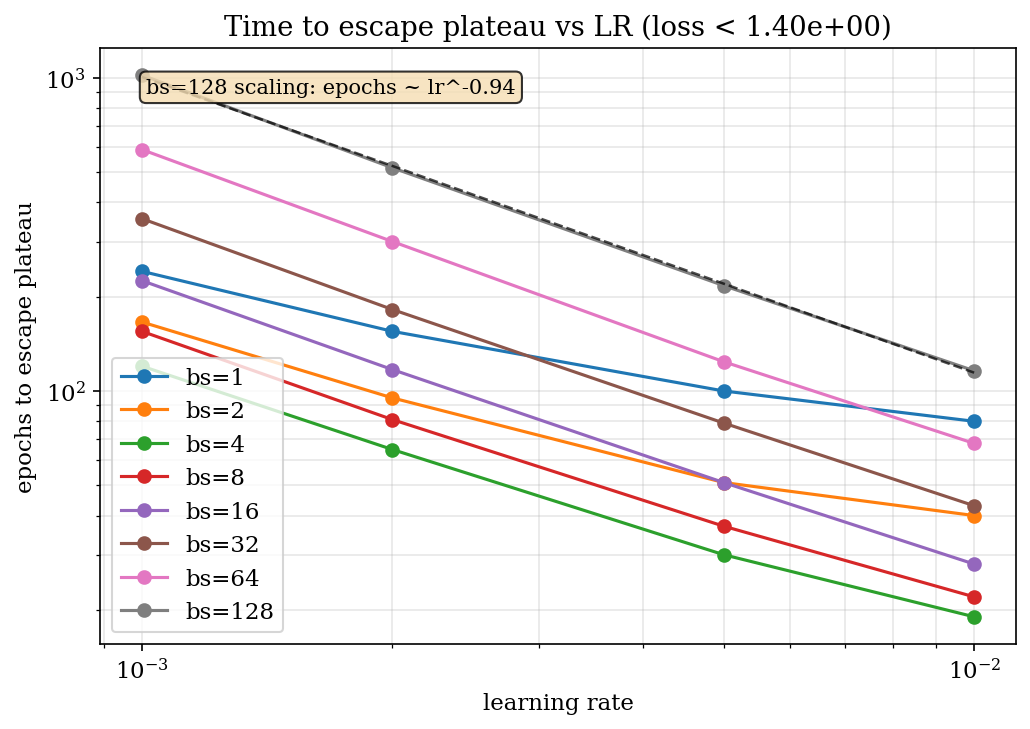
\includegraphics[width=0.42\linewidth]{figures/epochs_to_escape_vs_lr.png}
\caption{Epochs to escape the first plateau vs.\ learning rate (plateau-escape runs). Consistent with scaling $\propto 1/\mathrm{lr}$.}
\label{fig:escape_vs_lr}
\end{figure}

\begin{figure}[htbp]
\centering
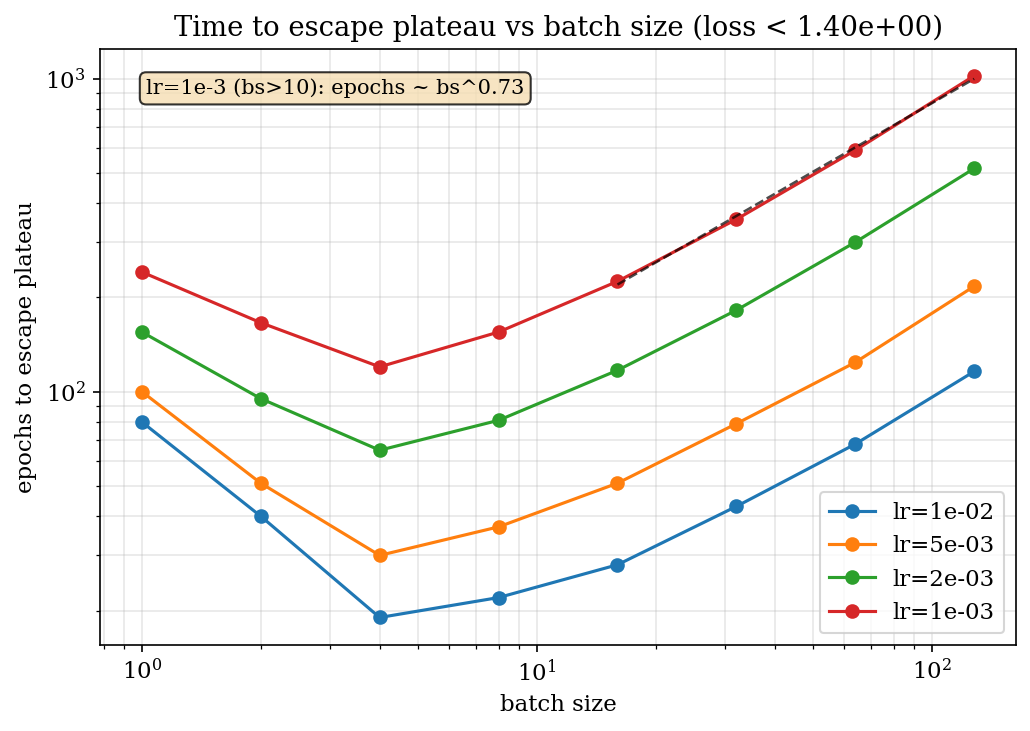
\includegraphics[width=0.42\linewidth]{figures/epochs_to_escape_vs_bs.png}
\caption{Epochs to escape vs.\ batch size. Small batch (1--4) escapes effectively; optimal/critical batch size in this setting.}
\label{fig:escape_vs_bs}
\end{figure}

\section{Figures: loss, fit, and partials before/after LR reduction}
\label{sec:figures}

We illustrate the \textbf{feature--landscape relation} with the runs described in Sections~\ref{sec:architecture} and \ref{sec:methodology} (factor $f_3$, $N=768$, batch size 8, depths $L=2$ and $L=3$). Figure~\ref{fig:loss_fit_L2} and Figure~\ref{fig:loss_fit_L3} show loss and fit before and after LR divides for $L=2$ and $L=3$. The \emph{sharp, nearly instantaneous} loss drops at each LR divide (visible in the curves) are the empirical signature of the picture in Section~\ref{sec:lr}: the landscape is a plateau with sharp, deep basins that become accessible when LR is reduced. The quality of the fit improves in step with these drops. Figure~\ref{fig:partial_L3} shows the evolution of \emph{partial functions} (channel outputs) before and after LR divides for $L=3$---the internal feature representation changes when the trajectory enters a sharper basin, making the link between landscape and feature learning directly visible. \textbf{Log-ratio trajectories} (channel dominance over training) further illustrate how LR and landscape shape specialization: at lr $2{\times}10^{-3}$, bs 4, the log-ratio trajectories exhibit \emph{divergence} globally by the end of training (Figure~\ref{fig:logratio_div}); at lr $2{\times}10^{-4}$, bs 4, they exhibit \emph{convergence} (Figure~\ref{fig:logratio_conv}). So the same architecture can either specialize (convergent log-ratios) or fail to stabilize (divergent) depending on the training regime, consistent with the valley--frequency picture. Channel-wise feature learning (log-ratio dynamics, spike specialization) is analyzed in a companion SciForDL submission (\texttt{features.tex}).

\begin{figure}[htbp]
\centering
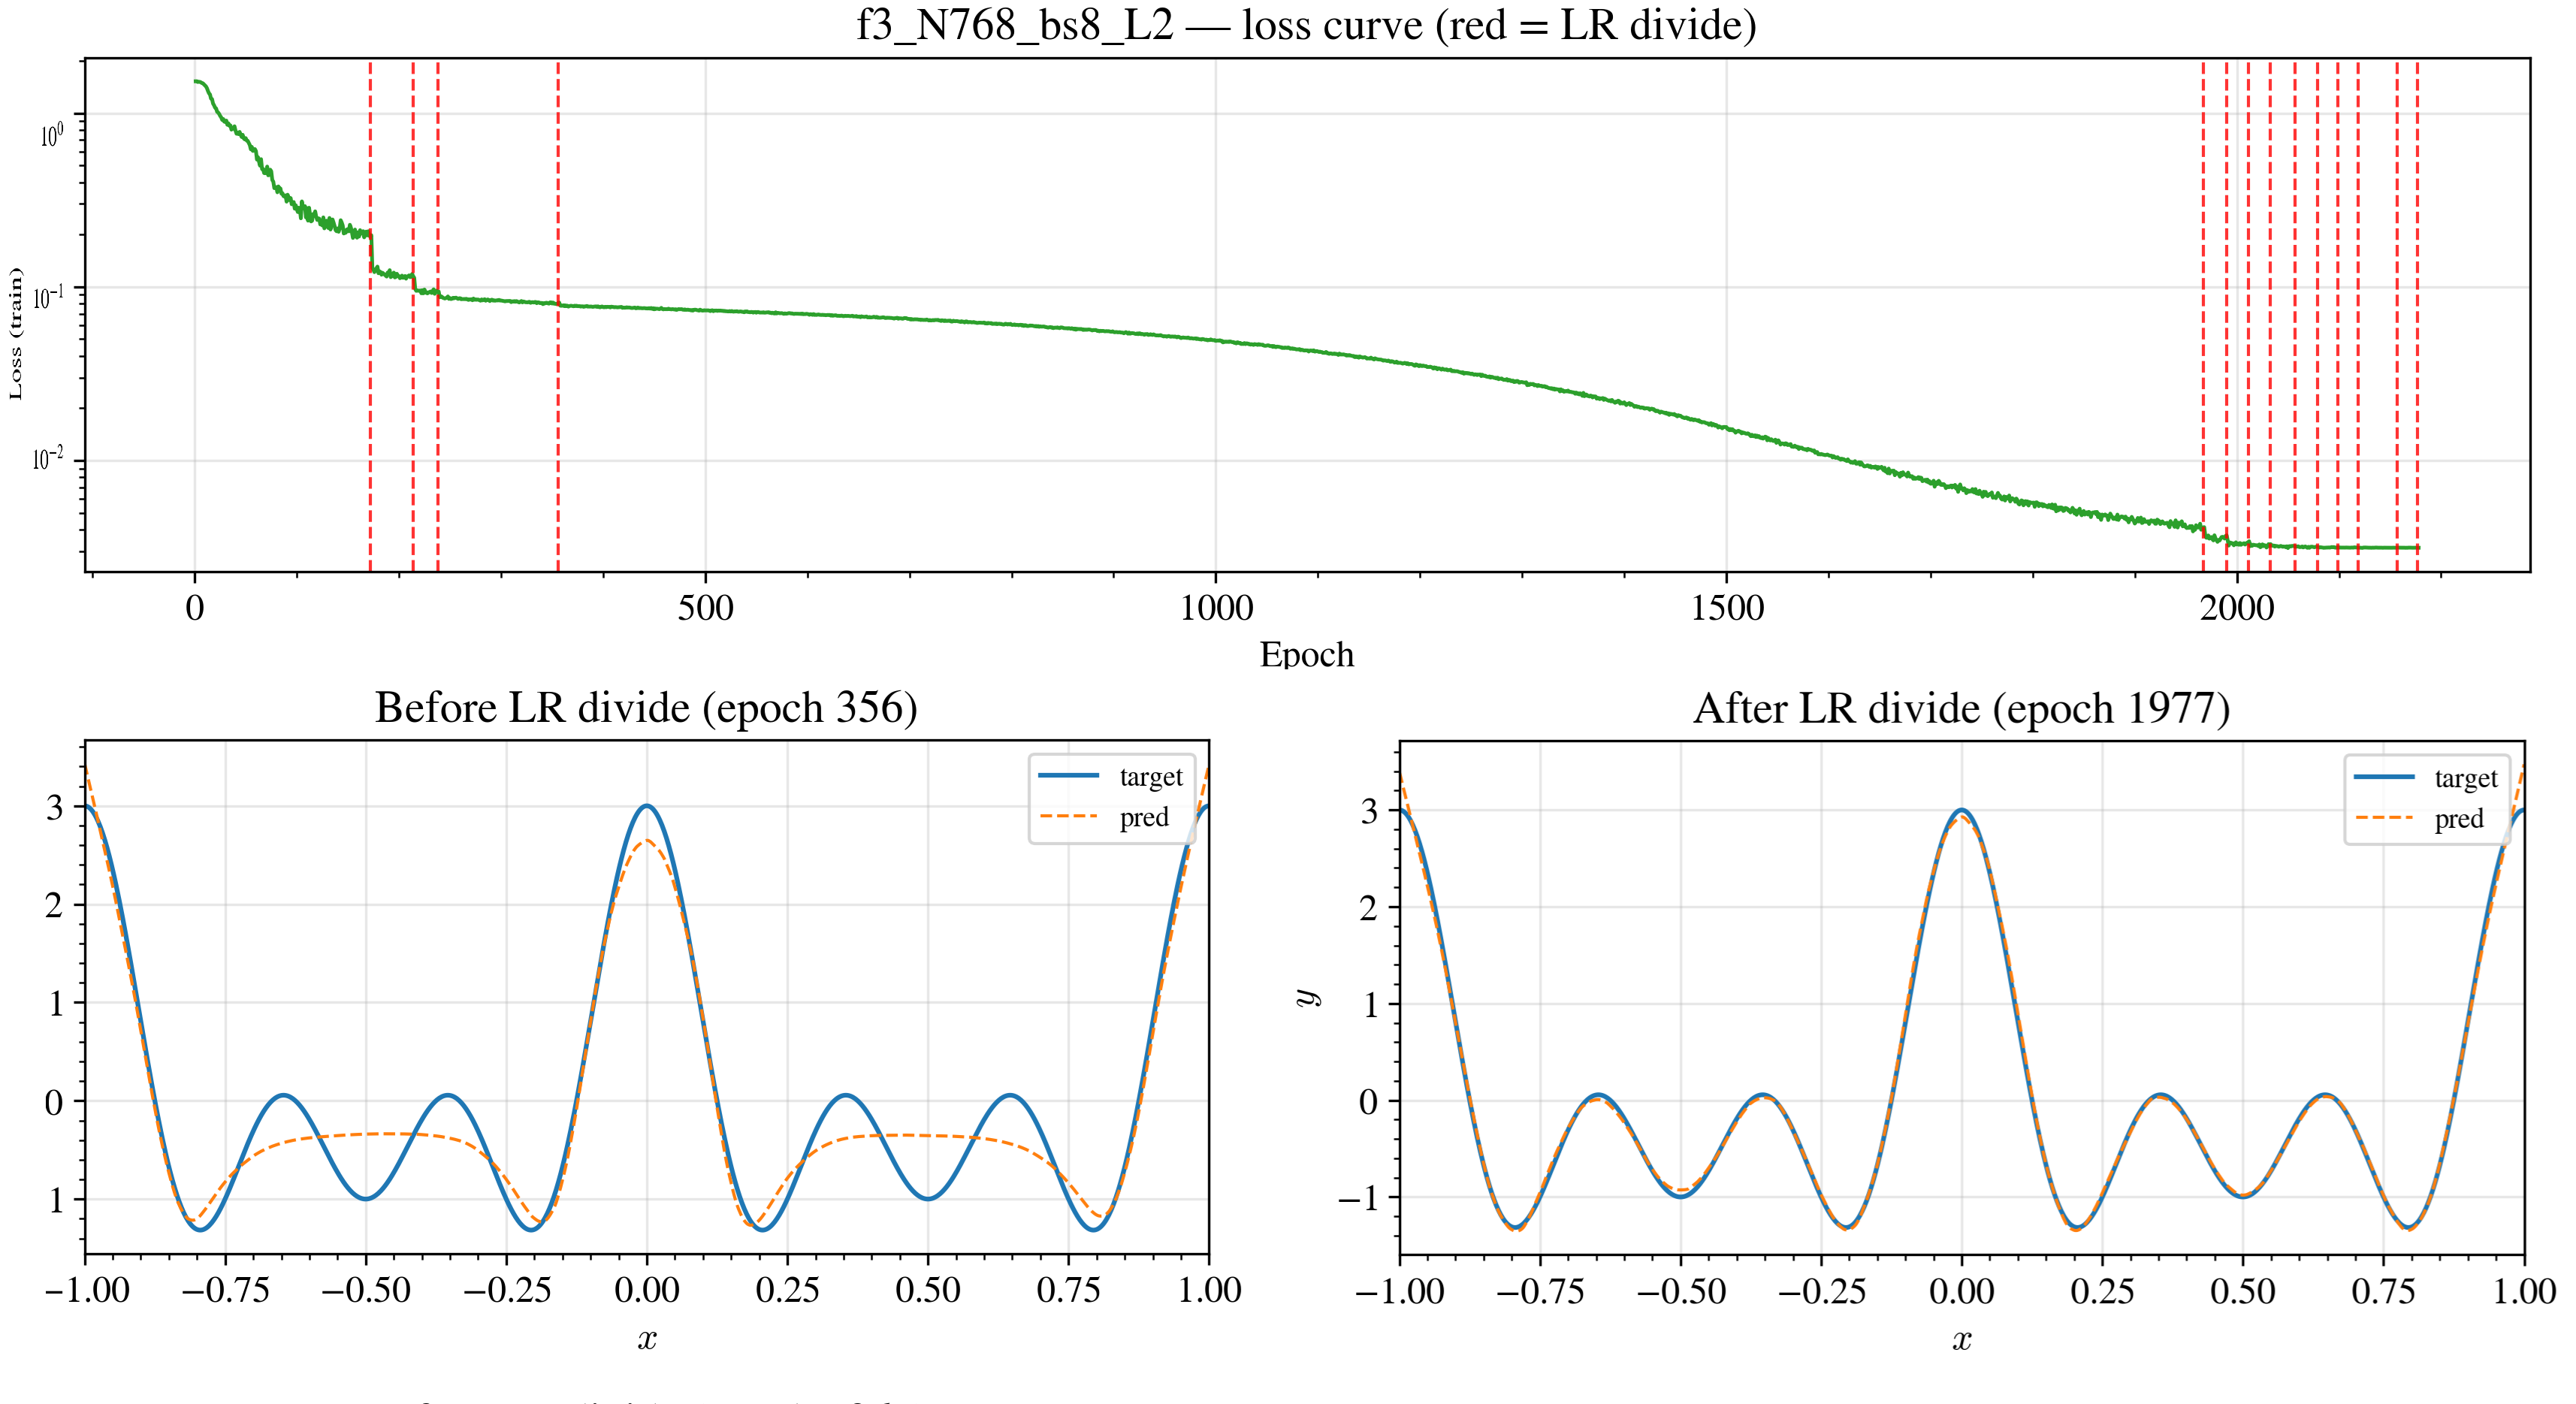
\includegraphics[width=0.42\linewidth]{figures/plot_loss_and_fit_before_after_lr_divides_L2.png}
\caption{Loss and fit before/after LR divides; $f_3$, $N=768$, bs=8, depth $L=2$.}
\label{fig:loss_fit_L2}
\end{figure}

\begin{figure}[htbp]
\centering
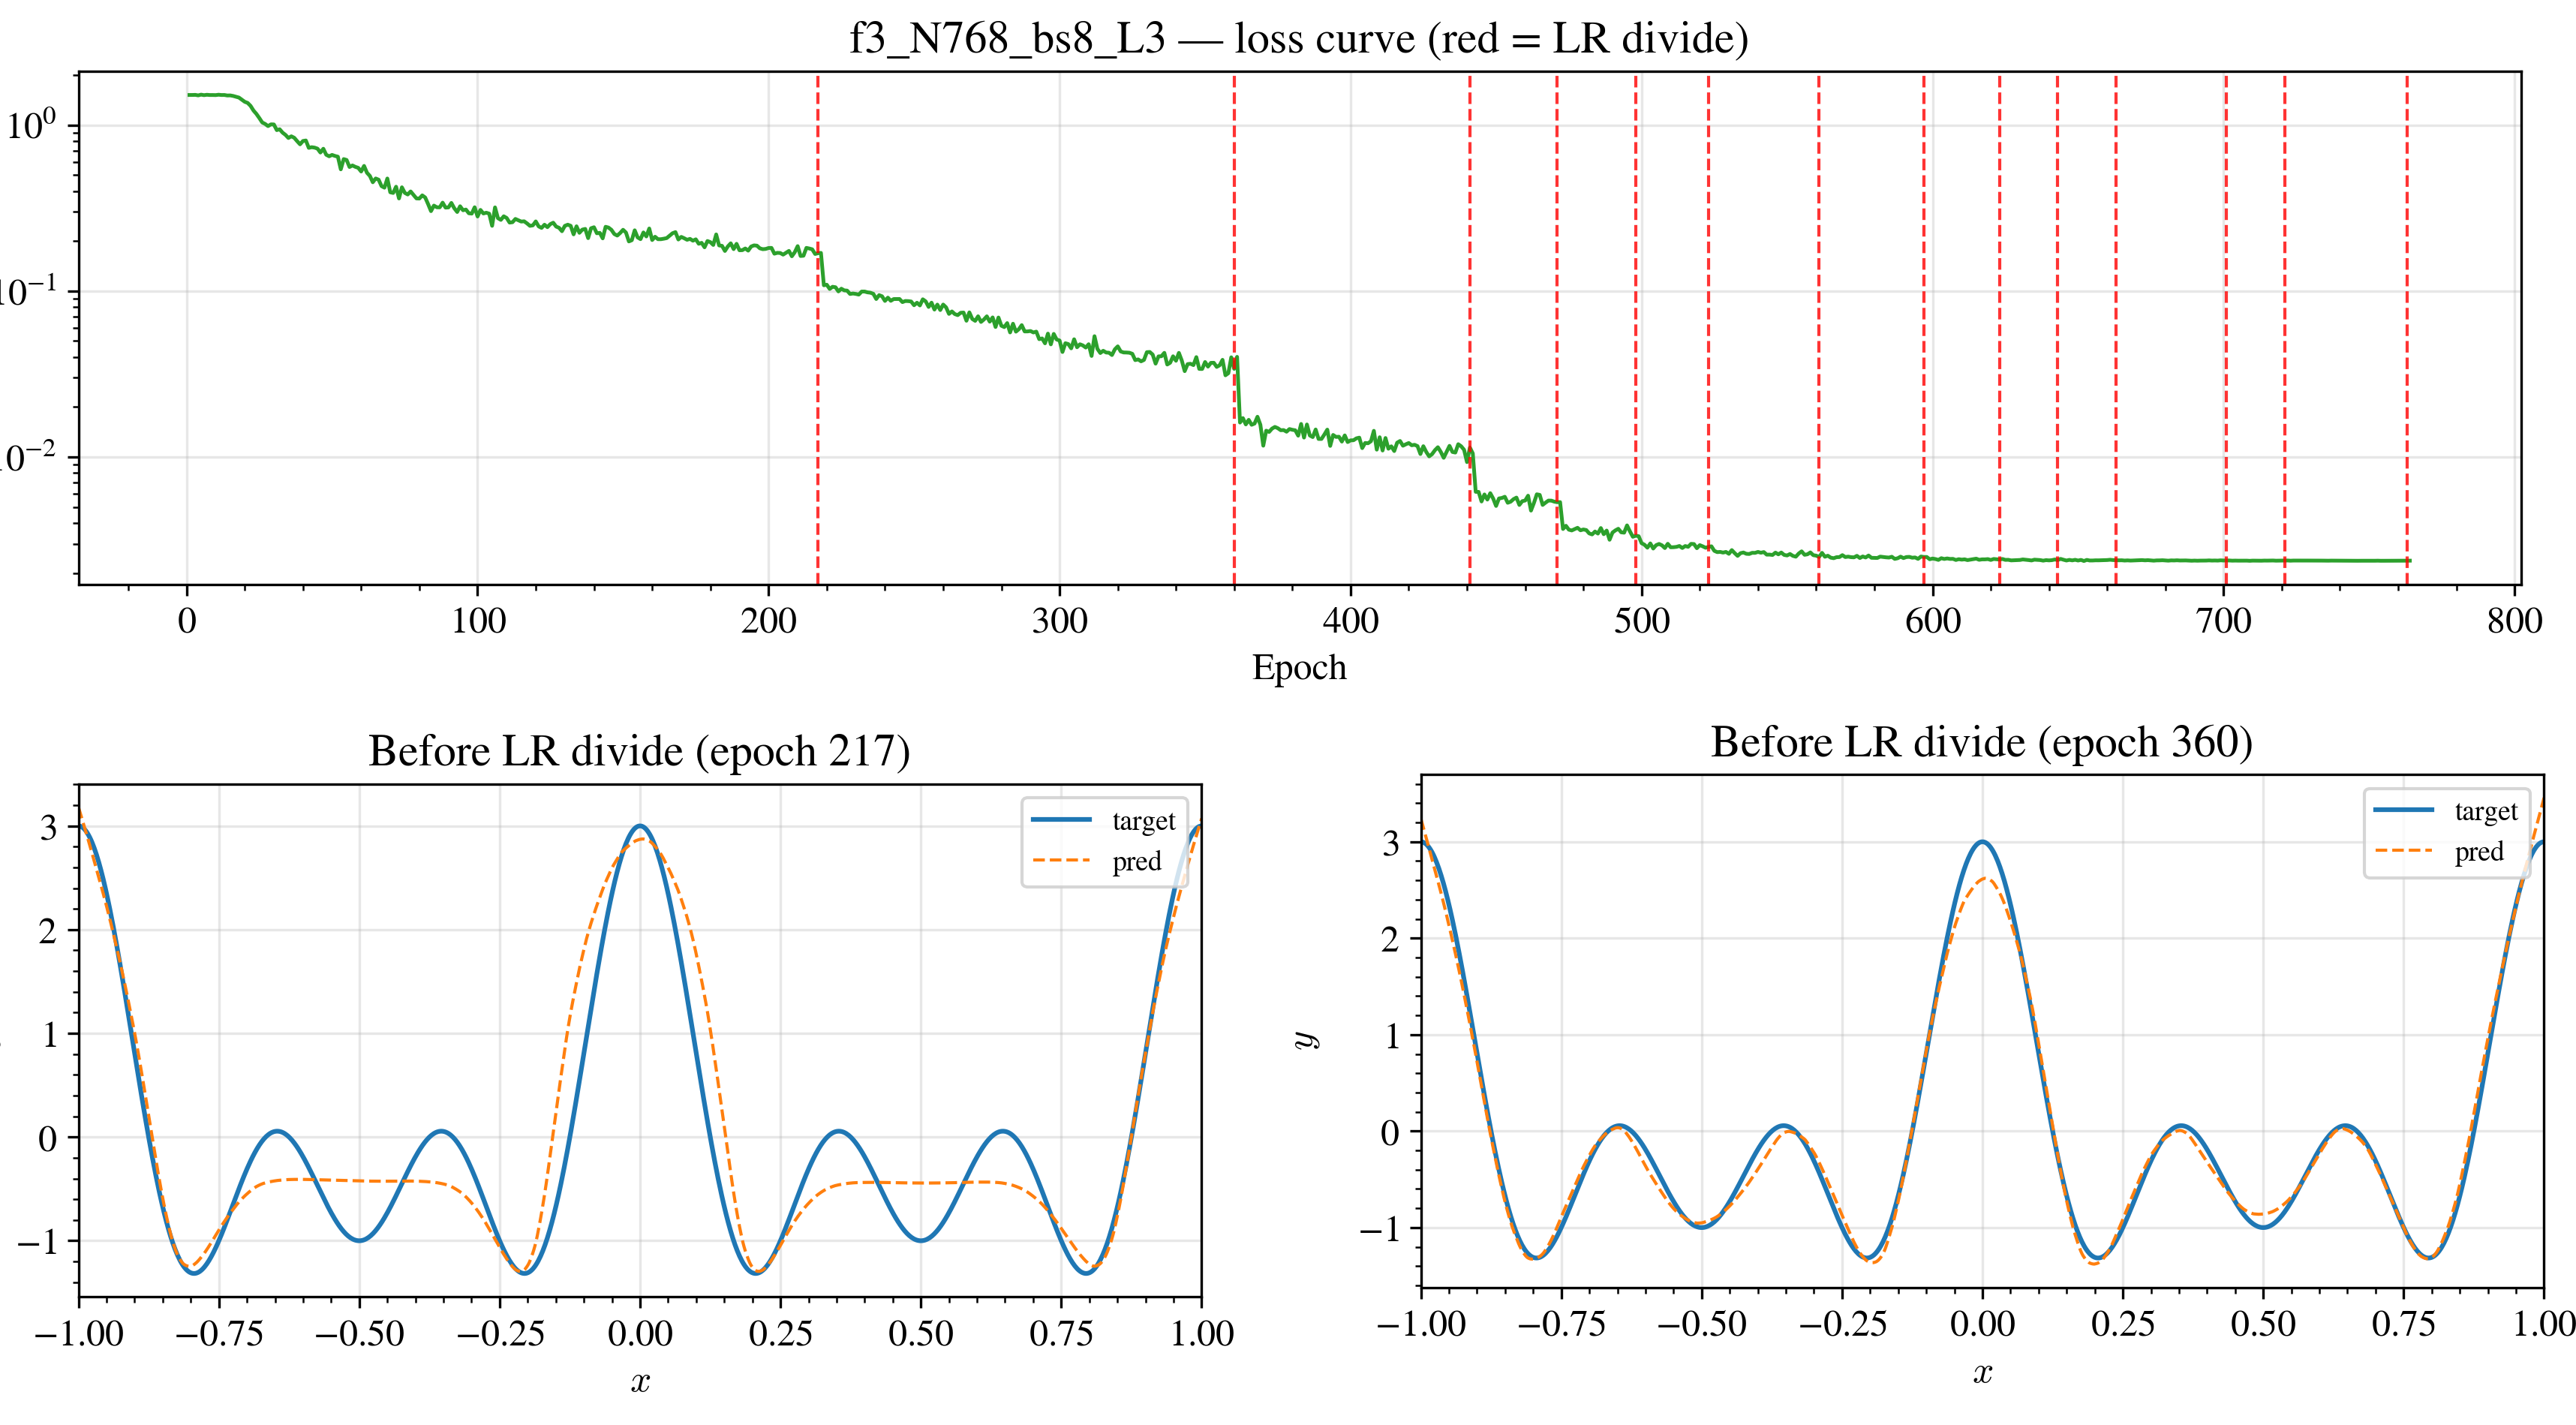
\includegraphics[width=0.42\linewidth]{figures/plot_loss_and_fit_before_after_lr_divides_L3.png}
\caption{Loss and fit before/after LR divides; $f_3$, $N=768$, bs=8, depth $L=3$.}
\label{fig:loss_fit_L3}
\end{figure}

\begin{figure}[htbp]
\centering
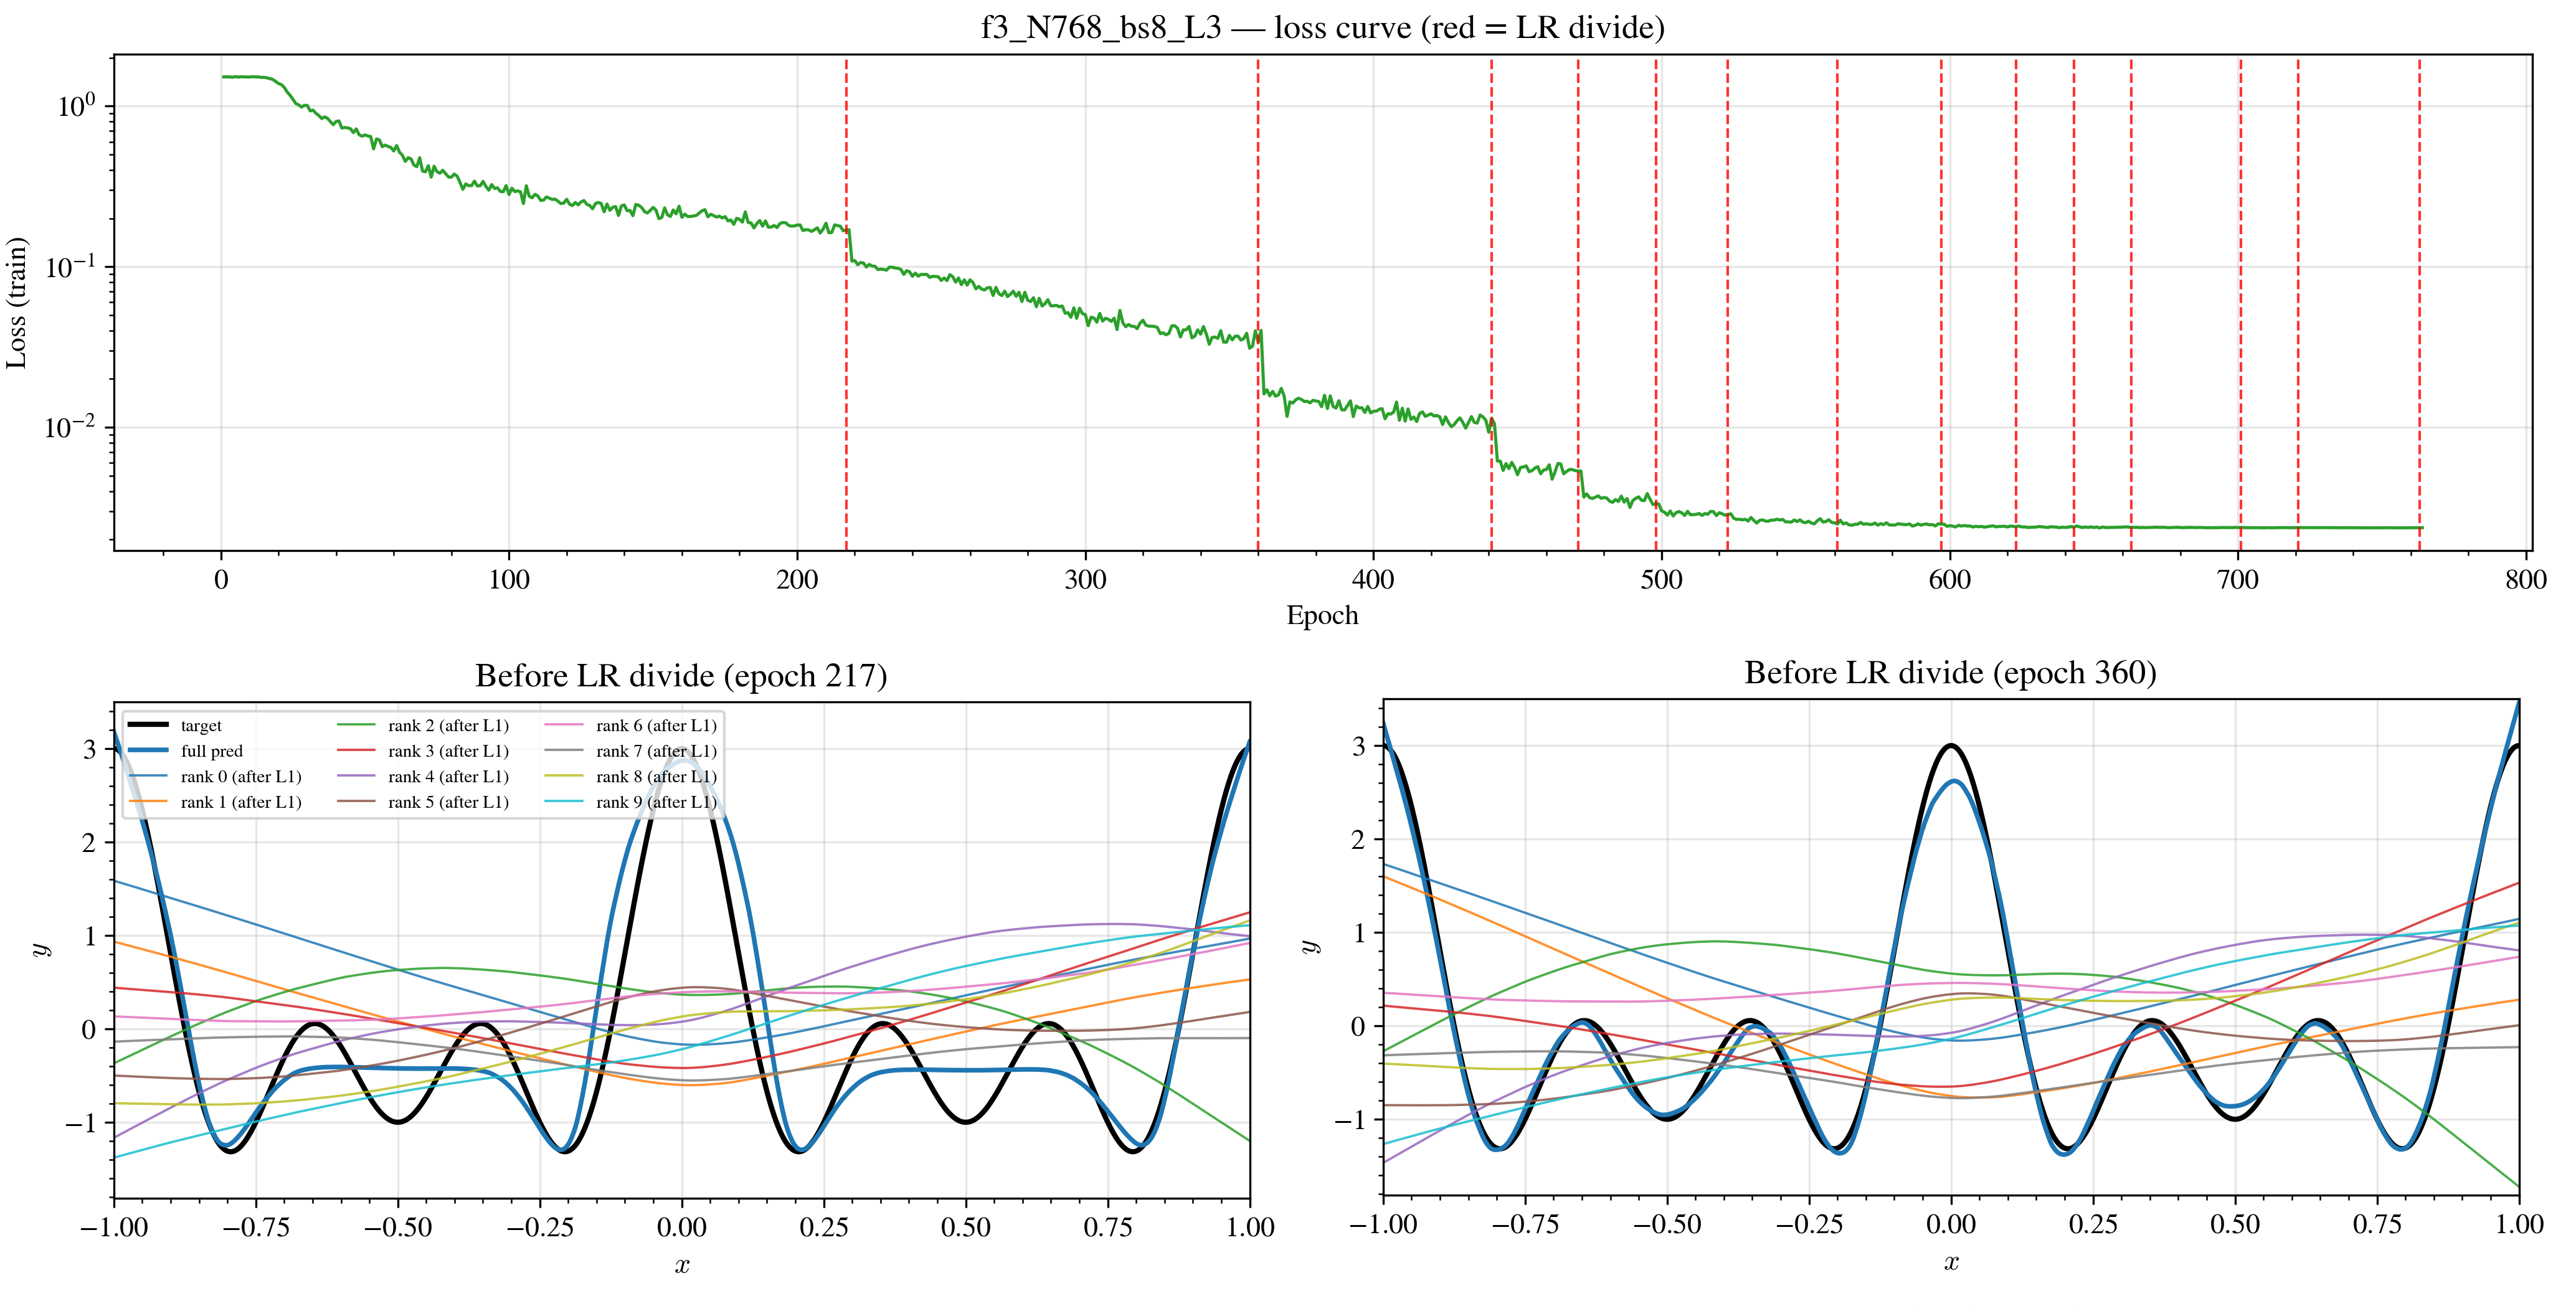
\includegraphics[width=0.42\linewidth]{figures/plot_partial_before_after_lr_divides_L3.png}
\caption{Partial functions before/after LR divides; $f_3$, $N=768$, bs=8, depth $L=3$.}
\label{fig:partial_L3}
\end{figure}

\begin{figure}[htbp]
\centering
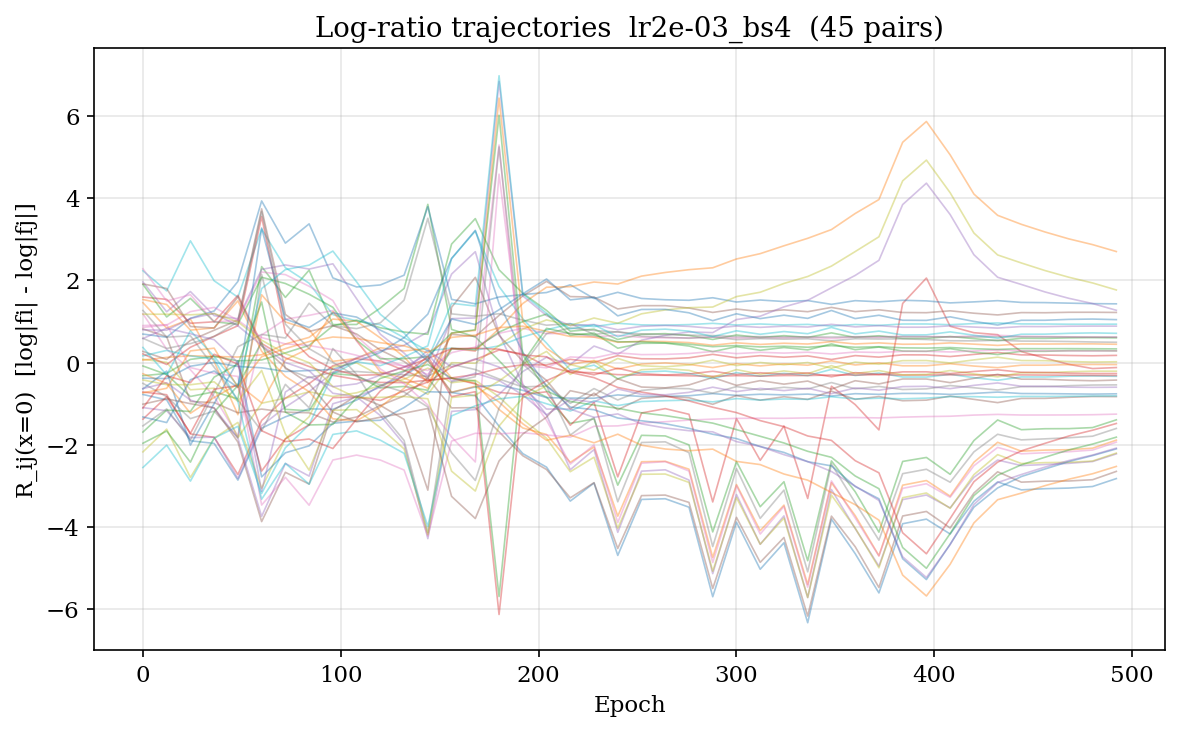
\includegraphics[width=0.42\linewidth]{figures/logratio_trajectories_lr2e-03_bs4_divergence.png}
\caption{Log-ratio trajectories (channel dominance over training); lr $2{\times}10^{-3}$, bs 4. Trajectories diverge globally by end of training.}
\label{fig:logratio_div}
\end{figure}

\begin{figure}[htbp]
\centering
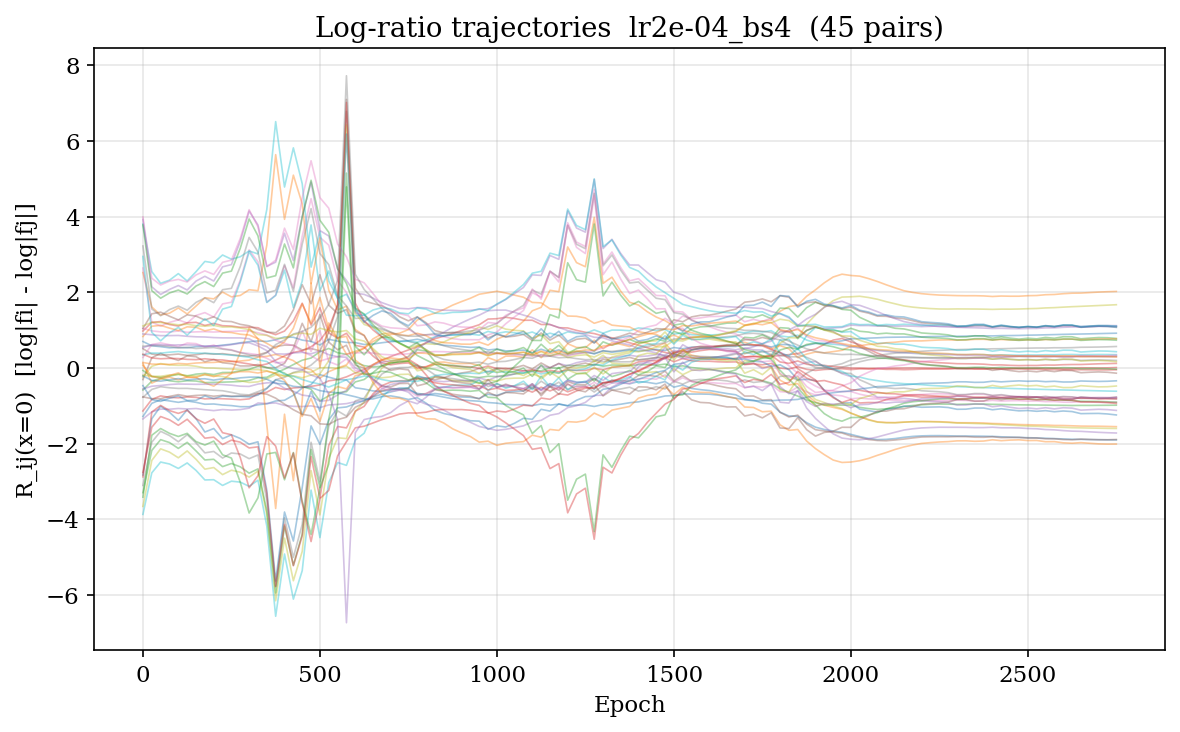
\includegraphics[width=0.42\linewidth]{figures/logratio_trajectories_lr2e-04_bs4_convergence.png}
\caption{Log-ratio trajectories; lr $2{\times}10^{-4}$, bs 4. Trajectories converge by end of training (stable specialization).}
\label{fig:logratio_conv}
\end{figure}

\section{Limitations}
\label{sec:limitations}

This study is restricted to 1D regression with the sum-of-cosines target and the MMNN architecture; we do not claim that the same feature--landscape relation holds in higher dimensions or for other architectures without further experiments. Observations on Adam (EOS jump, instability) and on self-similarity of training curves are qualitative; systematic replication over seeds and hyperparameters would be needed to establish robust scaling statements. In frequency/layer-scaling runs, very deep networks ($L=56$, $L=80$) can become unstable (huge test error or NaN), so depth scaling has a stability frontier in the current setup. The reported configs and script paths (including \texttt{run\_scaling\_law\_depth\_width.py}, \texttt{analyze\_baseline\_sweep.py}) are intended to make the methodology reproducible so that the relation can be verified or refuted.

\section{Conclusion}
\label{sec:conclusion}

We described the \textbf{relation between feature learning and the loss landscape} for low-rank neural networks in a controlled 1D setting. The two are tightly linked: (i) each plateau (or saddle) corresponds to a frequency to be learned and the dynamics are saddle-to-saddle, so the plateau--sharp--plateau loss structure corresponds to staged acquisition of frequency bands and to more oscillatory partial functions (e.g.\ mean minima per component increasing with depth); (ii) the landscape is a plateau with sharp, deep basins that are hard to enter unless the learning rate is small---at each LR divide the loss drops sharply and the trajectory enters such a basin, with loss, fit, and partial functions evolving together; (iii) low-rank structure (e.g.\ $2L$ spikes per layer $L$) yields a distinctive feature signature aligned with the hierarchical landscape. Within the stated scope (Section~\ref{sec:limitations}), understanding the loss landscape in these networks amounts to understanding how and when features are acquired. These observations support the SciForDL goal of building a scientific understanding of deep learning through reproducible experiments and explicit reporting of the relation between landscape geometry and learned representations.

\bibliography{iclr2026_conference}
\bibliographystyle{iclr2026_conference}

\appendix
\section{Appendix: Full experiment methodology and configs}
\label{app:methodology}

\subsection{Target and architecture (all experiments)}
Target: $y(x) = \sum_{k=1}^{\mathrm{factor}} \cos(2\pi k x)$ on $x \in [-1,1]$. MMNN: input/output dim 1; hidden rank $R$, width $W$; depth $L$ blocks (linear rank$\to$width, ReLU, linear width$\to$rank). fixWb = True (first linear frozen). $\mu$-parameterization; SGD momentum 0; gradient clipping max norm 1.0.

\subsection{Main figures (loss, fit, partials before/after LR divides)}
Runs used for Figures 3--5 (loss/fit L2, L3; partials L3): factor 3, $N_{\mathrm{train}}=768$, batch size 8, depths $L=2$ and $L=3$. Full parameterization:
\begin{itemize}
\item \textbf{Config name:} f3\_N768\_bs8\_L2, f3\_N768\_bs8\_L3.
\item \textbf{Data:} $N_{\mathrm{train}}=768$, batch\_size $=8$, factor $=3$.
\item \textbf{Architecture:} hidden\_width $=1024$, hidden\_rank $=10$, num\_layers $\in \{2,3\}$.
\item \textbf{Training:} num\_epochs $=10{,}000$; lr\_sequence: initial $0.01$, then divide by 2 at each reduction (25 steps); lr\_window $=10$, min\_epochs\_before\_reduce $=20$; stop if lr $< 10^{-6}$. Checkpoints: state before and 10 epochs after each LR divide.
\item \textbf{Optimizer:} SGD, momentum $0$, gradient clipping 1.0.
\end{itemize}

\subsection{Selected sumcos rerun configs (all)}
The following configs share the same LR schedule and architecture (width 1024, rank 10); only $N$, batch size, depth, and factor vary. Naming: f\{factor\}\_N\{n\_train\}\_bs\{batch\_size\}\_L\{num\_layers\}.

\begin{center}
\begin{tabular}{lccccl}
\hline
Config & $N$ & bs & $L$ & factor & Notes \\
\hline
f3\_N768\_bs8\_L2 & 768 & 8 & 2 & 3 & Main fig.\ loss/fit \\
f3\_N768\_bs8\_L3 & 768 & 8 & 3 & 3 & Main fig.\ loss/fit/partials \\
f3\_N768\_bs4\_L2 & 768 & 4 & 2 & 3 & \\
f3\_N768\_bs4\_L3 & 768 & 4 & 3 & 3 & \\
f3\_N768\_bs2\_L2 & 768 & 2 & 2 & 3 & \\
f3\_N768\_bs2\_L3 & 768 & 2 & 3 & 3 & \\
f3\_N768\_bs1\_L1 & 768 & 1 & 1 & 3 & \\
f3\_N768\_bs1\_L2 & 768 & 1 & 2 & 3 & \\
f3\_N384\_bs1\_L2 & 384 & 1 & 2 & 3 & \\
f3\_N384\_bs2\_L2 & 384 & 2 & 2 & 3 & \\
\hline
\end{tabular}
\end{center}

\subsection{Plateau-escape and log-ratio runs (Figures 1, 2, 6, 7)}
Plateau-escape runs train until loss $<$ threshold (escape); they record epochs to escape and log-ratio trajectories. Per run: fixed lr and batch size; factor 3, $N=768$, $L=3$, rank 10, width 1024. Naming: lr\{value\}\_bs\{batch\_size\} (e.g.\ lr2e-03\_bs4 = lr $2{\times}10^{-3}$, bs 4). Key params: escape\_threshold $=0.1$; max\_epochs 400--2000 depending on lr; log-ratio at $x=0$; checkpoint every 5--12 epochs. Figures 1--2: epochs to escape vs lr and vs batch size (sweep over lr $\in \{1{\times}10^{-2}, 2{\times}10^{-3}, 5{\times}10^{-3}, 1{\times}10^{-3}, 2{\times}10^{-4}, 5{\times}10^{-4}\}$, bs $\in \{1,2,4,8,16,32,64,128\}$). Figures 6--7: log-ratio trajectories for lr $2{\times}10^{-3}$ bs 4 (divergence) and lr $2{\times}10^{-4}$ bs 4 (convergence).

\subsection{Baseline sweeps (sumcos, rank 5/10/20)}
Target $\sum_{k=1}^{\mathrm{factor}} \cos(2\pi k x)$; factor $\in \{1,2,3,4,5\}$; $N = \mathrm{base} \times \mathrm{factor}$ with base $\in \{16,32,64,128,256\}$; batch sizes 1, 2, 4, 8, 16; depths $1 \ldots 2{\times}\mathrm{factor}$; max 10K epochs; adaptive LR (divide by 2 on stagnation); worked = test error $< 0.01$. Rank 5: 76 worked / 750; rank 10: 73 worked / 429. Small batch (1--4) outperforms 8, 16. Run naming: f\{f\}\_N\{n\}\_bs\{bs\}\_L\{L\}. Batch-size analysis and commands: BASELINE\_SWEEP\_SETUPS\_AND\_RANKS.md; INDEX\_LOGRATIO\_ESCAPE\_SCALING.md.

\subsection{Frequency/layer-scaling}
Multi-frequency target (freq multipliers 0.3--10); Adam, StepLR; ranks 10, 15, 25; layer counts per freq; 58 configs. Low freq (0.3, 0.6): test error $\sim 10^{-6}$--$10^{-5}$; high freq (1.5+): no convergence; very deep ($L=56$, 80): blow-up or NaN. CSV and summary: \texttt{--train} then \texttt{--analyze}.

\subsection{Symmetry comparison (Figure~\ref{fig:mlp-asymmetry})}
Same architecture as low-rank runs but with RF/low-rank removed (full-rank MLP, fixWb = False): 8 layers, width $n=1024$, effective rank $r=20$, target $f(x)=\cos(f_1\pi x^2)-0.8\cos(f_2\pi x^2)$ on $[-1,1]$ with $(f_1,f_2)=(144,48)$; $N=4\mathrm{k}$ train, 10k epochs, Adam lr $0.001$, batch 100, StepLR $\gamma=0.9$ every 100 steps. Plots show channel partials at layers 7 and 16; asymmetry about $x=0$ is visible. Low-rank (RF-LR) runs with same hyperparameters preserve symmetry (see \texttt{icml\_sgdadamlandscapedynamical/tofill.tex}, Sec.~5.3).

\subsection{Stable baseline}
Target cos $2\pi x$; $N = \mathrm{width} = 1024$, rank 10, $L=2$, batch 4; 250 epochs; SGD lr 0.01, AdaptiveStagnation (sequence 0.01, 0.005, 0.001, 0.0005, 0.0001). Best: momentum 0.7, test error $\sim 1.9{\times}10^{-6}$.

\subsection{Script and document index}
Training: \texttt{run\_selected\_sumcos\_configs.py} (selected rerun); \texttt{run\_scaling\_law\_depth\_width.py} (baseline, baseline-sweep, baseline-sweep-rank5, baseline-sweep-rank N, baseline-sweep-expcos, train, analyze). Plateau escape and log-ratios: \texttt{run\_plateau\_escape.py}. Analysis: \texttt{analyze\_baseline\_sweep.py} (--sumcos, --sumcos-rank5, --sumcos-rank20, --expcos). Docs: BASELINE\_SWEEP\_SETUPS\_AND\_RANKS.md (batch-size and run naming); INDEX\_LOGRATIO\_ESCAPE\_SCALING.md (scaling law and sweep references); idea.md, experiments/partialfunctionanalysis/ for further detail.

\newpage
\section{Science of DL Improvement Challenge Submission}

\subsection{What model are you targeting?}
Low-rank neural networks (MMNNs, RF-LR) for 1D regression on hierarchical Fourier targets (e.g.\ sum of cosines). We target the \textbf{relation between feature learning and the loss landscape}: how the geometry of the loss (plateaus, sharp drops, basins) connects to what the network learns internally (channel partials, frequency bands, oscillatory structure).

\subsection{How do your results contribute—or could potentially contribute—to understanding these models?}
We document that feature learning and the loss landscape are tightly linked: (i) each plateau/saddle corresponds to a frequency to be learned and dynamics are saddle-to-saddle; (ii) the landscape is a plateau with many sharp, deep basins that are hard to enter unless LR is small---at each LR divide the loss drops sharply (as in the provided figures) and the trajectory enters such a basin; (iii) observables such as mean minima per component and $2L$ spikes per layer $L$ bridge landscape and feature learning. This contributes a concrete, empirical picture of how landscape geometry and learned representations relate in low-rank nets.

\subsection{How do you expect your submission to influence future work?}
The feature--landscape relation can be tested systematically (multiple seeds, architectures, metrics); scaling laws (plateau escape, batch size) and the link to feature-learning diagnostics (log-ratio, minima counts) can be refined; and the same methodology can be extended to other tasks and architectures to see how general the relation is.

\end{document}
